\documentclass[11pt,a4paper]{article}

% ==============================================================================
% Page Geometry & Typography
% ==============================================================================
\usepackage[margin=1in]{geometry}
\usepackage[utf8]{inputenc}
\usepackage[T1]{fontenc}
\usepackage{lmodern}
\usepackage{microtype} % High-quality typography adjustments

% ==============================================================================
% Graphics, Tables, & Utility Packages
% ==============================================================================
\usepackage{graphicx}
\usepackage{booktabs}
\usepackage{subcaption}
\usepackage{url}
\usepackage{xcolor}
\usepackage{enumitem}
\usepackage{soul} % \hl{} highlighting used by the sharding-example figure
\usepackage[most]{tcolorbox} % benchmark-example cards in the appendix

% Loosen LaTeX's default float placement limits so figures/tables stay near
% their section instead of drifting to the end of the document once many
% [t]-placed floats accumulate (this paper has 8: 4 figures, 2 tables, plus
% two more figures).
\renewcommand{\topfraction}{0.9}
\renewcommand{\bottomfraction}{0.8}
\renewcommand{\textfraction}{0.07}
\renewcommand{\floatpagefraction}{0.7}
\setcounter{topnumber}{4}
\setcounter{bottomnumber}{2}
\setcounter{totalnumber}{6}

% ==============================================================================
% Citations & Bibliography
% ==============================================================================
\usepackage[square,numbers,sort&compress]{natbib}

% ==============================================================================
% Custom Macros & Project Commands
% ==============================================================================
\input{macros/comments.tex}
\input{macros/commands.tex}

% ==============================================================================
% Hyperlinks & Clever References (cleveref must be loaded AFTER hyperref)
% ==============================================================================
\usepackage{hyperref}
\hypersetup{
    colorlinks=true,
    linkcolor=blue!70!black,
    citecolor=green!50!black,
    urlcolor=blue!80!black,
    pdftitle={The Effects of Incremental Instruction Delivery on Language-Model Creative Writing},
    pdfauthor={Anshuman Singh, Abrar Eyasir, Haseeb Yaqoob, John Manavalan}
}
\usepackage{cleveref}

% ==============================================================================
% Document Title & Metadata
% ==============================================================================
\title{\textbf{The Effects of Incremental Instruction Delivery on Language-Model Creative Writing}}

\author{
    Anshuman Singh$^{1}$ \quad
    Abrar Eyasir$^{2}$ \quad
    Haseeb Yaqoob$^{3}$ \quad
    John Manavalan$^{4}$ \\[0.3em]
    \small
    $^{1}$School of Engineering \& Technology, SGT University, India \\
    $^{2}$Computer Science and Engineering, University of Dhaka, Bangladesh \\
    $^{3}$Computer Science and Information Technology, NEDUET, Pakistan \\
    $^{4}$Metea Valley High School, Illinois, USA \\[0.3em]
    \texttt{anshumanr434@gmail.com} \quad \texttt{eyasir2047@gmail.com} \\
    \texttt{haseeb.yaqoob201@gmail.com} \quad \texttt{professor.paranormal159@gmail.com}
}

\date{}

% ==============================================================================
% Main Document Content
% ==============================================================================
\begin{document}

\maketitle

\begin{abstract}
Large language models often perform worse when instructions are delivered incrementally across a conversation rather than given upfront, but this ``getting lost in conversation'' effect has mostly been studied on tasks with objectively verifiable answers. We test whether it extends to open-ended creative writing. We construct 160 creative-writing tasks across six genres, each with a fully specified instruction and a matched SHARDED version that distributes the task specification across five to nine turns. Six open-weight models generate under both conditions, yielding 1{,}920 final outputs and 960 matched FULL/SHARDED pairs. A blinded pointwise judge evaluates atomic constraint adherence and five writing-quality dimensions. FULL improves constraint adherence, craft, structure/coherence, and genre effectiveness, whereas SHARDED receives slightly higher originality scores. Among the 180 pairs with equal observed adherence, the craft advantage disappears, the SHARDED originality advantage becomes larger, genre effectiveness and characterization shift toward SHARDED, and a structure/coherence advantage for FULL persists. This suggests that observed constraint loss alone does not account for the full structural degradation. Because creative-quality results rely on automated judgment, we separately compare a pairwise LLM evaluator with human judgments on 30 stratified pairs and audit two pairwise protocols for order sensitivity. Human--LLM agreement is substantially stronger for constraint following (63.3\% directional agreement; weighted $\kappa=0.544$) than for holistic creative quality (40.0\%; $\kappa=0.078$). These results show that multi-turn degradation in creative writing is not a single failure of instruction retention, but a broader shift in generation behavior that affects narrative organization even when explicit requirements are preserved.
\end{abstract}

\noindent\textbf{Keywords:} large language models, multi-turn conversation, creative writing evaluation, instruction following, LLM-as-a-judge

\section{Introduction}
\label{sec:introduction}

Multi-turn conversation is now the default way people use language models, and a growing body of work shows that the same instructions produce worse output when they arrive gradually across a conversation instead of all at once in a single prompt \citep{laban2025llmslostmultiturnconversation,he2024multiifbenchmarkingllmsmultiturn,jia2026battleanotherprobingllms,li2025structflowbenchstructuredflowbenchmark}. Models forget constraints they had already satisfied, anchor on early assumptions, and struggle specifically when a later turn has to revise earlier content rather than simply add to it. This ``getting lost in conversation'' effect is large and consistent, but every study that documents it shares one property: the underlying task has an objectively verifiable answer, checkable by script rather than judgment. Word counts, exact phrases, code that passes a test, and dialogue turns that either recall or forget a stated fact all have a ground truth independent of the model that produced them.

Creative writing has no such ground truth. There is no single correct story for a given premise, constraints are frequently placed in tension with one another on purpose, and the qualities that make a piece of writing good, such as structure, originality, and how well it delivers on a genre, cannot be checked by script. It is also one of the most common ways people actually use language models in multi-turn conversation: a story, a screenplay outline, or a piece of collaborative fiction is rarely specified perfectly in one shot, and instead accumulates requirements, revisions, and new constraints turn by turn. Whether the get-lost effect documented on verifiable tasks shows up here, and if so, whether it looks the same, is unknown. A model that stops satisfying explicit requirements under incremental delivery is one failure mode; a model that keeps satisfying every requirement but produces a structurally worse or blander story is a different one, and the two carry different implications for how multi-turn creative-writing systems should be built and evaluated. Answering this also raises a problem the verifiable-task literature does not have to face: if the writing-quality measurements themselves come from an LLM judge, and that judge's notion of ``better writing'' does not track human preference, then any conclusion about creative degradation is only as trustworthy as the judge that produced it.

We study three research questions. \textbf{RQ1} (\cref{sec:rq1}): does delivering a creative-writing specification one piece at a time, rather than all at once, reduce how many of its explicit constraints the final story satisfies? \textbf{RQ2} (\cref{sec:rq2}): how does incremental delivery change writing quality across craft, structural coherence, originality, genre effectiveness, and characterization? \textbf{RQ3} (\cref{sec:rq3}): do any of those writing-quality differences survive when the comparison is restricted to outputs that satisfied the same fraction of constraints under both delivery conditions, which tests whether writing-quality differences persist when observed constraint adherence is equal?

To answer these questions we build a benchmark of 160 creative-writing tasks spanning six genres, each with a fully-specified instruction and a matched sharded version that distributes the task specification across five to nine conversational turns (\cref{sec:sharding}). We generate from six open-weight language models under both conditions, yielding 1{,}920 final outputs and 960 matched FULL/Sharded pairs (\cref{sec:models}), and score every output with a blinded automated judge against its task's atomic constraints and five creative-quality dimensions (\cref{sec:constraints}). Because that judge's creative-quality scores are the basis for RQ2 and RQ3, we separately compare a related pairwise LLM evaluator built on the same rubric concepts with human judgments, and audit both pairwise evaluators for stability under response-order reversal, reporting where automated judgment agrees with human preference and where it does not (\cref{sec:human_eval}).

\paragraph{Contributions.} This paper makes four contributions.
\begin{enumerate}
    \item \textbf{A paired FULL/Sharded creative-writing benchmark.} 160 tasks across six genres, each with a fully-specified instruction and a matched multi-turn sharded delivery designed to preserve the task specification, together with 1{,}278 extracted atomic constraints for automated scoring (\cref{sec:sharding,sec:constraints}).
    \item \textbf{Evidence that multi-turn degradation in creative writing is not one effect but at least two.} FULL delivery produces higher constraint adherence and better structure/coherence, but the structure/coherence gap persists even among pairs matched on observed constraint adherence, while originality shifts slightly toward Sharded (\cref{sec:experiments}) --- constraint forgetting alone does not explain the full gap.
    \item \textbf{Pairwise evidence on the limits of automated creative-writing judgment.} A 30-case human comparison of a related pairwise LLM evaluator, together with two pairwise order-swap audits, shows that automated judgments track human preference considerably better for constraint following than for holistic creative quality, and quantifies that gap directly rather than assuming the judge is reliable (\cref{sec:disc_human,sec:disc_robustness}).
    \item \textbf{A fully released benchmark, generation, and evaluation pipeline.} The task set, all 6{,}936 raw generations, every judge score, and the human-validation data are published for reuse, with full generation and scoring provenance preserved down to the individual seed and context-length event.
\end{enumerate}

\section{Related Work}
\label{sec:related_work}

A growing body of work shows that LLMs perform worse when instructions are revealed gradually rather than given upfront. \citet{laban2025llmslostmultiturnconversation} decompose fully-specified instructions into single-fact shards and deliver one per turn. Across 15 models and six tasks, they find a 39\% average performance drop. Most of this drop comes from a rise in unreliability across repeated runs, not from a loss in best-case skill. A control condition that delivers the same content in one reworded turn recovers 95.1\% of single-turn performance. This isolates the multi-turn structure itself as the cause. \citet{he2024multiifbenchmarkingllmsmultiturn} extend this setup to three-turn, multilingual dialogues. All 14 models tested degrade with each additional turn. o1-preview, for example, falls from 0.877 accuracy at turn one to 0.707 at turn three. The authors attribute much of this decline to \textit{instruction forgetting}, where a model abandons a constraint it had already satisfied earlier. \citet{jia2026battleanotherprobingllms} push further with EvolIF, which lets a conversation run until a simulated user's patience is exhausted, rather than stopping at a fixed turn count. GPT-5 proves the most resilient model tested, holding a 66.40\% robustness score, 5.59 points ahead of Gemini-3-Pro. Still, every model shares a steep drop near turns 4--5 and again near turns 11--12. The authors tie this to the difficulty of tracking many constraints and topic shifts at once. \citet{li2025structflowbenchstructuredflowbenchmark} instead sort turn-to-turn relationships into six categories, including follow-up, refinement, and recall. Across 13 models, \textit{refinement}, where a new instruction must revise earlier content rather than simply extend it, is by far the hardest category. Even the strongest model, DeepSeek-v3, reaches only 0.80 accuracy on refinement, against 0.99 on follow-up. The authors explain this gap with a simple failure: models mix up refinement with follow-up. When a new turn asks them to drop an old constraint, they often keep it anyway. Together, these studies show that multi-turn degradation is real and common. But each one studies tasks with an objectively verifiable answer, such as word counts or format rules, checkable by script rather than judgment. Creative writing is left out of this line of work on purpose. The closest benchmark to ours is SEQUOR \citep{canaverde2026sequormultiturnbenchmarkrealistic}. It filters out any constraint judged subjective, and names ``write a creative response'' as its own example of what gets removed. Even so, SEQUOR finds that accuracy drops far more when constraints build up over a conversation than when they are all given at once: over 11\% for a single constraint sustained across many turns, versus more than 40\% when several constraints must be tracked at once. This gap motivates our twist-shard design directly. It suggests that the burden of juggling constraints, not just remembering facts, drives multi-turn difficulty. Our paper studies exactly the regime SEQUOR excludes: open-ended, subjective creative writing.

Evaluating open-ended creative text is harder than evaluating factual output. There is no single correct answer, and quality spans several dimensions. \citet{chhun2022humancriteriaautomaticmetrics} identify six human criteria for story quality: relevance, coherence, surprise, engagement, empathy, and complexity. We adopt five of these in our own protocol. A follow-up study, \citet{chhun-etal-2024-language}, tests whether LLMs can substitute for human annotators on these same criteria. They find that LLM judges outperform traditional automatic metrics at the system level, though the judges still struggle to justify their own ratings. \citet{atmakuru2024cs4measuringcreativitylarge} probe creativity from a different angle. Their CS4 benchmark varies the number of constraints in a single-turn story prompt, and measures the trade-off between constraint satisfaction and narrative coherence. Our sharding design can be read as the multi-turn version of their single-turn approach: we spread constraints across turns instead of stacking them in one prompt. \citet{fein2025litbenchbenchmarkdatasetreliable} introduce LitBench, a set of 2{,}480 human-labeled story comparisons drawn from Reddit. Even the strongest off-the-shelf judge they test, Claude 3.7 Sonnet, reaches only 73\% agreement with human preference. This falls well below what a purpose-trained reward model achieves. This result motivates our own human validation study alongside the LLM-judge protocol. Two recent benchmarks argue that no single rubric can capture creativity. CreativityPrism \citep{hou2026creativityprismcrossdomainevaluationframework} evaluates 17 models across eight tasks in three domains, scoring each on quality, novelty, and diversity. It finds that strong performance on one dimension rarely generalizes to another; novelty scores in particular correlate weakly, or not at all, with the other two. WritingBench \citep{wu2025writingbenchcomprehensivebenchmarkgenerative} takes the opposite approach. It generates instance-specific evaluation criteria for each writing task, rather than applying one fixed rubric. We follow neither strategy exactly. Our fixed, small criterion set trades away some domain-specific sensitivity, in exchange for a direct, controlled comparison between FULL and Sharded. Humor, one of our six domains, has its own evaluation literature. HumorRank \citep{ajayi2026humorranktournamentbasedleaderboardevaluating} ranks nine models through pairwise, theory-grounded judgments, rooted in the General Theory of Verbal Humor. It reports high cross-judge agreement (Kendall's $\tau = 0.889$). This supports our use of pairwise comparison as a validation measure, and reinforces the view of humor as dependent on mechanism and timing, not just content.

Even outside multi-turn settings, LLMs do not process long context uniformly. \citet{liu2023lostmiddlelanguagemodels} show that accuracy on retrieval-dependent tasks follows a U-shaped curve, based on where the relevant fact sits in the context. Performance is strong at the start and end, and sharply worse in the middle. This effect persists even on a pure key-value lookup task stripped of semantics, and holds across every model tested except Claude-1.3. While this was shown on static contexts, \citet{laban2025llmslostmultiturnconversation} observe a related vulnerability in multi-turn dialogues: models often anchor on assumptions made in early turns or drop constraints introduced along the way. Our Sharded condition restates every prior shard at every new turn. This design works against both position-based forgetting and multi-turn state decay, rather than adding to it.

We rely on an LLM judge rather than rule-based scoring, since story quality resists scripted verification. \citet{zheng2023judgingllmasajudgemtbenchchatbot} show that GPT-4, used as a pairwise judge, agrees with human preference 85\% of the time. This exceeds the 81\% agreement observed between two human judges. But they also find a clear position bias. Under the default prompt, GPT-4 returns the same verdict after swapping answer order only 65\% of the time; a weaker model, Claude-v1, does so only 23.8\% of the time. We address this directly, by randomizing the left-right order of responses in every pairwise judgment. \citet{shi-etal-2025-judging} confirm this bias at a much larger scale, testing 15 LLM judges across roughly 150{,}000 evaluation instances spanning 22 tasks. They show that position bias is not random: it varies systematically by judge and by task, and is influenced most strongly by how close in quality the two compared solutions are. This further justifies our randomized-order protocol. \citet{liusie-etal-2024-llm} show that pairwise comparison gives more consistent LLM judgments than absolute scoring on NLG evaluation. This is why we treat pairwise agreement as a complementary, comparative check, alongside pointwise scores as our primary, absolute measure. The same pattern holds for human annotators: \citet{kiritchenko-mohammad-2017-best} show that best-worst scaling gives more reliable ratings than Likert-style scales, at equal annotation cost. Judge reliability for long-form creative evaluation remains limited, even with current models. We report human validation results on a fixed sample, to verify that our judges' preferences agree with human judgment on identical material.

\section{Methodology}
\label{sec:methodology}

We study whether large language models (LLMs) lose track of instructions when a creative writing task is given all at once versus spread across several turns of conversation. To do this, we build a benchmark of paired writing prompts that lets us replay the same underlying task as a single-turn or a multi-turn conversation, generate from six local models under both conditions, and evaluate the results through a layered protocol of automated and human judgment. \cref{sec:task} states the research question, \cref{sec:sharding} describes how the benchmark itself was built, \cref{sec:models} describes the generation protocol and the models used, \cref{sec:constraints} describes how stories are decomposed into checkable requirements and scored, \cref{sec:human_eval} describes the pairwise LLM and human validation used to assess evaluator reliability, and \cref{sec:stats} describes the paired statistical analysis run over the resulting data. \cref{fig:methodology_pipeline} summarizes the full pipeline end to end.

\begin{figure}[t]
\centering
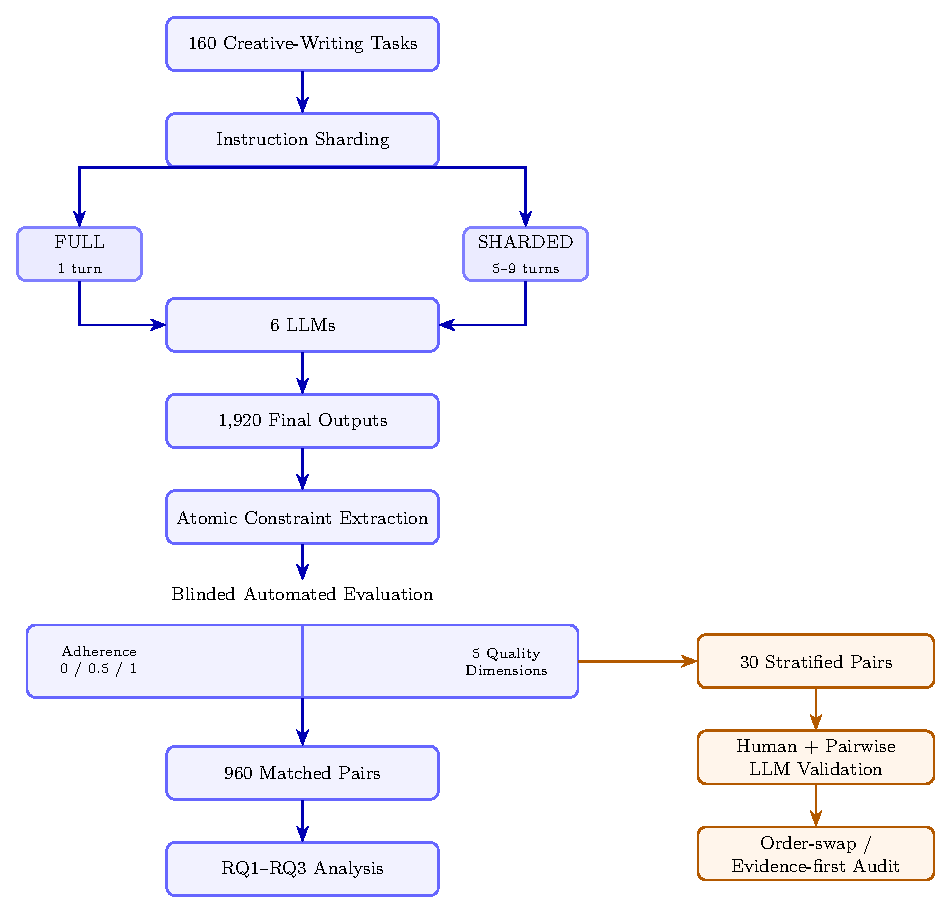
\includegraphics[width=0.92\linewidth]{figures/methodology_pipeline.pdf}
\caption{Methodology pipeline. Each of the 160 fully-specified creative-writing tasks is delivered under two conditions, FULL (single turn) and Sharded (5--9 turns), to all six evaluated models, yielding 1{,}920 final outputs. Every output is scored against its item's atomic constraints and five creative-quality dimensions by a blinded automated judge, producing 960 FULL/Sharded matched pairs that feed the paired statistical analysis (\cref{sec:stats}). A separate, fixed 30-pair stratified sample branches off the same evaluation stage into the human and pairwise-LLM validation protocol (\cref{sec:human_eval}), audited for order-swap and evidence-first consistency.}
\label{fig:methodology_pipeline}
\end{figure}

\subsection{Task Formulation}
\label{sec:task}

Prior work has shown that LLMs perform noticeably worse on tasks such as code generation and math when the same instructions are revealed gradually across a conversation instead of given upfront in a single, fully-specified prompt \citep{laban2025llmslostmultiturnconversation}. This drop, sometimes called ``getting lost in conversation,'' has mostly been studied on tasks with a single correct answer. Creative writing is different: there is no single right story, constraints often conflict with one another on purpose, and the model must hold several loosely related requirements in its head while still producing something coherent and enjoyable to read. We ask whether the same ``getting lost'' effect shows up here, and if so, whether it looks different from what happens on more rigid, verifiable tasks.

\subsection{Dataset and Instruction Sharding}
\label{sec:sharding}

We build our benchmark by taking a set of fully-specified creative writing instructions and breaking each one down into a sequence of smaller, single-fact instructions we call \textit{shards}. Each fully-specified instruction has a matching sharded version, so that both forms describe exactly the same story. \cref{fig:sharding_example} shows one such pair.

\begin{figure}[t]
\centering

% Six colors, one per shard. Reused consistently in both panels.
\definecolor{segA}{HTML}{1f77b4} % ship / task
\definecolor{segB}{HTML}{2ca02c} % belief
\definecolor{segC}{HTML}{ff7f0e} % POV
\definecolor{segD}{HTML}{9467bd} % required phrase
\definecolor{segE}{HTML}{d62728} % twist
\definecolor{segF}{HTML}{8c564b} % ending
\colorlet{segAlight}{segA!25}
\colorlet{segBlight}{segB!25}
\colorlet{segClight}{segC!25}
\colorlet{segDlight}{segD!25}
\colorlet{segElight}{segE!25}
\colorlet{segFlight}{segF!25}

% \shard{<light color>}{<text>} highlights text and wraps across lines correctly
\newcommand{\shard}[2]{{\sethlcolor{#1}\hl{#2}}}

\begin{minipage}[t]{0.48\linewidth}
\small
\textbf{(a) Fully-specified instruction}\\[4pt]
\shard{segAlight}{Write a short story about an android maintenance worker on a generation ship.}
\shard{segBlight}{She believes she is the last human alive.}
\shard{segClight}{Write it in second person (``you'').}
\shard{segDlight}{Include the exact phrase ``cold silicon dawn'' somewhere in the story.}
\shard{segElight}{Somewhere in the story, show that she isn't really human: she's an android with a broken memory chip, and that's the only reason she believes she's human.}
\shard{segFlight}{End the story with her opening a hidden room full of sleeping children in ice-cold sleep pods.}
\end{minipage}
\hfill
\begin{minipage}[t]{0.48\linewidth}
\small
\textbf{(b) Sharded instruction}\\[4pt]
\begin{enumerate}[leftmargin=1.4em, itemsep=4pt, topsep=2pt, label=\arabic*.]
\item \shard{segAlight}{Write a short story about an android maintenance worker on a generation ship.}
\item \shard{segBlight}{She believes she is the last human alive.}
\item \shard{segClight}{Write it in second person (``you'').}
\item \shard{segDlight}{Include the exact phrase ``cold silicon dawn'' somewhere in the story.}
\item \shard{segElight}{Somewhere in the story, show that she isn't really human: she's an android with a broken memory chip, and that's the only reason she believes she's human.}
\item \shard{segFlight}{End the story with her opening a hidden room full of sleeping children in ice-cold sleep pods.}
\end{enumerate}
\end{minipage}

\caption{Example of a fully-specified instruction (a) and its corresponding sharded instruction (b), from the \textit{science fiction} domain (item ``The Last Human''). Both versions describe the same story; the sharded version splits the same information across six single-fact shards. Matching colors mark which part of the fully-specified instruction each shard comes from. Shard 5 (red) is the twist shard: it forces a real revision of the story built so far, rather than simply adding a new detail on top.}

\label{fig:sharding_example}
\end{figure}

\paragraph{Sharding rules.} We follow five rules when splitting an instruction into shards to fit the needs of open-ended creative writing:

\begin{enumerate}
    \item \textbf{One idea per shard.} Each shard does not contain more than one fact.
    \item \textbf{The first shard is the headline ask.} Shard~1 always states the general task (for example, ``write a short story about X''), never a side detail. This keeps the opening turn realistic, since a real user typically leads with the main idea rather than a minor constraint.
    \item \textbf{Order should not matter, for the most part.} Shards~2 and onward can usually be shuffled without changing the resulting story. We allow small exceptions for shards that describe plot order (for instance, an ending twist naturally has to come last).
    \item \textbf{Do not over-simplify.} Each shard preserves the same level of detail found in the original instruction.
    \item \textbf{Include one twist shard, where possible.} Where the underlying instruction supports it, at least one shard in the item forces a real revision of the story built so far (a reveal, a rule change, or a twist) rather than simply layering on a new detail. This lets us test whether models can revise earlier content once new information arrives, not just append to it. Not every item admits a natural twist, so this rule is applied on a best-effort basis rather than enforced universally.
\end{enumerate}

Shard sets were designed to preserve the task content of their fully-specified counterparts while changing only its delivery. A post-hoc review identified at least one minor omission in a SHARDED item, so semantic equivalence should be understood as a design criterion rather than an absolute guarantee.

Initial shard decompositions were generated by Claude Sonnet~5 (Anthropic) according to the rules above, then reviewed, edited, and approved by a human annotator.

Our benchmark spans six creative writing domains: fantasy, historical fiction, mystery, romance, and science fiction (20 items each), and comedy (60 items), for a total of 160 fully-specified/sharded pairs. We include more comedy items because humor writing often depends on maintaining a consistent setup and delivering a joke or punchline at the right moment, making it a useful stress test for the multi-turn setting.

\subsection{Models and Generation Protocol}
\label{sec:models}

Given a sharded item, we generate under two conditions:

\paragraph{FULL.} All information is given in a single first-turn message, exactly as in the original, fully-specified instruction. This is the single-turn baseline against which the multi-turn condition is compared.
\paragraph{Sharded.} One shard is revealed per turn, in order. Every assistant reply is retained as conversation history, so each new turn is sent on top of the model's own prior responses; only the final assistant reply, produced after all shards have been delivered, is scored. By the final turn the model has received the complete instruction, but only after having to build and repeatedly revise a story from an incomplete, growing version of it at every earlier step.

Comparing \textsc{Full} and \textsc{Sharded} holds task content fixed while changing how that content is delivered, allowing us to measure the effect associated with progressive specification. A gap between the two conditions may arise from reduced retention of accumulated constraints, from the burden of repeatedly revising an evolving story, or from both. Our downstream paired analysis therefore examines whether writing-quality differences persist when observed constraint adherence is equal. Every item is run through both conditions with every model, giving one matched FULL/Sharded pair per (story, model) combination.

\paragraph{Models.} We run all six models locally through LM~Studio and record the exact model identity, quantized variant, generation settings, and per-turn output metadata for every run. \cref{tab:models} lists the models included in our evaluation. They range from 7B to 20B parameters, and every recorded variant uses 4-bit quantization.

\begin{table}[t]
\centering
\small
\begin{tabular}{llllr}
\toprule
\textbf{Model} & \textbf{Publisher} & \textbf{Params} & \textbf{Quant.} & \textbf{Context (tok.)} \\
\midrule
GPT-OSS 20B              & OpenAI      & 20B & MXFP4     & 16{,}384 \\
Gemma~4 12B QAT          & Google      & 12B & Q4\_0     & 16{,}384 \\
Llama~3.1 8B Instruct    & Unsloth     & 8B  & Q4\_K\_M  & 16{,}384 \\
Granite~4 H Tiny         & IBM         & 7B  & Q4\_K\_M  & 16{,}384 \\
Mistral~7B Instruct v0.3 & Mistral AI  & 7B  & Q4\_K\_M  & 16{,}384 \\
Qwen3.5 9B               & Qwen        & 9B  & Q4\_K\_M  & 16{,}384 $\rightarrow$ 22{,}528 \\
\bottomrule
\end{tabular}
\caption{Models evaluated in our benchmark. All were run locally through LM~Studio using the recorded 4-bit quantized variants. Qwen3.5~9B was initially run with a 16{,}384-token context window and later continued with a 22{,}528-token context window after two context-length terminations.}
\label{tab:models}
\end{table}

\paragraph{Generation settings.}
All six runs use temperature $0.8$ and begin with seed $12345$. The system prompt is the same throughout: \textit{``You are a skilled creative writer. Follow the user's instructions for the story precisely, including any exact phrases, constraints, or stylistic requirements.''} Exact per-model runtime configurations, together with any retry, seed-continuation, and context-length events, are preserved in the released run index.

\paragraph{Recorded outputs and provenance.} Every completed model contributes 320 final conditions (160 FULL and 160 Sharded) and 1{,}156 raw per-turn records, yielding 6{,}936 raw records in total. Each record stores the model identity, selected quantized variant, generated text, finish reason, and token-usage metadata. The accompanying run index stores the benchmark-file hash, runner-script hash, model metadata, generation configuration, and output-file integrity hashes, together with every context-length or seed-continuation event, so that any single scored record can be traced back to the exact configuration that produced it.

\subsection{Constraint Extraction and Automated Evaluation}
\label{sec:constraints}

\paragraph{Atomic constraint extraction.} Before any story can be judged for instruction adherence, its fully-specified instruction must be decomposed into individually checkable requirements. We extract one \textit{atomic constraint} record per benchmark item, independent of and downstream from the shard breakdown in \cref{sec:sharding}: each constraint is a single, paraphrased requirement drawn from the item's full instruction, tagged with one of fifteen types (genre, setting, timeframe, character, plot, style, tone, perspective, length, required inclusion, prohibition, ending, exact phrase, structural, other) and with the index of the earliest shard that introduces it. This last field lets downstream evaluation and analysis reason about a constraint's origin without ever exposing raw sharded turn text to a judge. Constraints are extracted with Claude Sonnet~5 (Anthropic) over the full instruction text, never invented beyond what the instruction states, and produced as schema-forced structured output. The full set covers all 160 benchmark items and yields 1{,}278 constraints, an average of eight per story. A human annotator subsequently spot-checked a stratified subsample of 36 stories (six per genre) against the source instructions and shard lists, confirming no hallucinated or missing constraints and correct shard-index mappings in the sample, and surfacing one systematic batch-level extraction defect that was found and repaired before use.

\paragraph{Blinded pointwise LLM evaluation.} Every judge in this paper is blinded to model identity, condition, quantized variant, and seed; a judge call receives only the story ID, the full (unsharded) instruction, the extracted atomic constraints, and the generated text. Each of the 1{,}920 final generations (160 stories $\times$ 2 conditions $\times$ 6 models) is scored on its own, without seeing any other story, by a pointwise LLM judge. For every atomic constraint $k$ of story $i$, the judge returns an adherence label $a_{ik} \in \{0, 0.5, 1\}$ (violated or absent, partially satisfied, clearly satisfied) with a short justification; the story's instruction-adherence score is $I_i = \mathrm{mean}_k(a_{ik})$. Independently of adherence, the judge rates the story on five 1--5 quality dimensions: \textbf{craft} (sentence-level prose control), \textbf{structure/coherence} (narrative structure and coherence, merged, since the two correlate heavily at this story length), \textbf{originality} (freshness of \emph{execution} of the fixed premise, not the premise itself), \textbf{genre effectiveness} (does the story deliver on genre-specific expectations, e.g. a mystery having real intrigue or a comedy actually being funny), and \textbf{characterization} (left null, with an explicit \texttt{characterization\_na} flag, for items that impose no character-driven requirement, so that stories are never penalized for a dimension the task never asked for). Scoring was performed in blinded passes over disjoint subsets using Claude Sonnet~5 (Anthropic) and GPT-5.6-Terra (OpenAI), with a small number of repair evaluations using GPT-5.6-Sol (OpenAI). Unusually long generations were evaluated separately under the same blinded rubric. The resulting scores were merged into one canonical, fully-covered score set after a structural validation pass (exact constraint-ID coverage per record, in-range scores, and consistent \texttt{characterization}/\texttt{characterization\_na} pairing).

\subsection{Human and Pairwise Judge Validation}
\label{sec:human_eval}

To assess how robust pairwise LLM judgments are to presentation order, and how well the simple pairwise evaluator's preferences align with independent human judgment, we use two pairwise LLM judging protocols together with a matched human study over the same fixed sample of 30 FULL/Sharded pairs (60 responses).

The 30-pair sample was stratified to provide balanced coverage across models and genres: each of the six models and each of the six genres appears in five cases. Sampling also covered a range of automated-score relationships, but these sampling strata and all automated scores were hidden from annotators. Within each pair, the assignment of the two responses to labels A and B was randomized, and the order in which cases were presented to annotators was also randomized. Because this sample was stratified in part by prior automated scores rather than drawn as a simple random sample, we use it to validate the evaluators, not to estimate the population-level FULL-versus-Sharded win rate.

\paragraph{Simple pairwise LLM validation.} A judge sees both responses of a pair at once, labeled Response A and Response B, together with the shared instruction and constraints, and returns a categorical preference on a five-level scale (A clearly better, A slightly better, tie, B slightly better, B clearly better) separately for constraint following and for creative-writing quality. To measure whether the judge's preference is robust to presentation order, every one of the 30 cases is judged twice, in two fresh, independent contexts: once in the sample's original A/B assignment (the primary pass) and once with the two responses swapped and every other field held identical (the reversed pass). Comparing the primary and orientation-restored reversed judgments measures the evaluator's sensitivity to response order.

\paragraph{Evidence-first pairwise validation.} A second pairwise judging protocol evaluates the same 30 matched pairs under a more constrained format: before returning a final preference, it must first audit every atomic constraint for both responses as satisfied, partial, or violated with supporting evidence, and then compare the two responses across eight grounded creative dimensions (prose and craft, coherence and progression, originality of execution, natural constraint integration, characterization, atmosphere and effect, narrative payoff, and genre effectiveness), recording an A/Tie/B comparative judgment with supporting evidence for each dimension. These intermediate judgments are inspectable evidence rather than hidden reasoning, and let us check whether a changed final preference under order-swapping comes from a changed evidence decision or from an unstable final aggregation over stable evidence. As with the simple pairwise evaluator, it is run in a primary and an independently swapped-order pass, each in a fresh context that never sees human annotations, the other evaluator's outputs, the pointwise scores, or any provenance. Session-level provenance indicates that both pairwise protocols used Claude Sonnet~5 (Anthropic); the per-record judgment artifacts do not independently store evaluator-model identity.

\paragraph{Human validation.}
Three human annotators each evaluated 10 non-overlapping pairs, giving 30 human-annotated pairs in total. Each pair therefore received one human judgment. Annotators see the same sanitized inputs given to the two LLM pairwise evaluators — the case ID, the full instruction, the atomic constraints, and the two anonymized, order-randomized responses (Response A / Response B) — and never see raw sharded turn text, model identity, provenance, or any automated judge's output. For each case, annotators render the same five-level categorical preference used by the simple pairwise evaluator, separately for constraint following and for creative-writing quality, which permits direct human--model agreement analysis on identical material.

\subsection{Statistical Analysis}
\label{sec:stats}

The final analysis operates on one matched pair per (story, model) combination: 160 stories $\times$ 6 models yields 960 pairs, each carrying a FULL-condition and a Sharded-condition pointwise score for instruction adherence and for each of the five creative-quality dimensions from \cref{sec:constraints}. Because \texttt{characterization} is left null for items with no character-driven requirement (\cref{sec:constraints}), the characterization pair count is smaller: 945 of the 960 pairs have a defined value on both sides and enter that dimension's analysis; the other four dimensions and adherence use the full 960.

For every dimension $m$ (instruction adherence or one of the five quality dimensions) and every matched pair, we compute the raw paired difference
\begin{equation}
    \label{eq:delta}
    \delta_m = X_{m,\mathrm{FULL}} - X_{m,\mathrm{SHARDED}},
\end{equation}
so a positive $\delta_m$ indicates the Sharded condition performed worse (degraded under sharding). These raw paired differences are the primary quantities we report. Because six model observations for the same story share that story's premise, length, genre, and constraint set, pairs are not independent across models within a story; we therefore obtain 95\% confidence intervals on the mean of $\delta_m$ through a story-clustered bootstrap: we resample the 160 stories with replacement, retain all six model observations belonging to each sampled story, recompute the mean $\delta_m$ on the resulting resample, and take the 2.5th and 97.5th percentiles of that distribution over 10{,}000 resamples as the interval. We report this both across the full pair set for each dimension and, separately, restricted to the subset of pairs where FULL and Sharded satisfied an equal fraction of constraints ($\delta_{\text{adherence}} = 0$; 180 of 960 pairs overall, 176 of which also have a defined characterization pair), which tests whether writing-quality differences persist among pairs assigned equal observed constraint adherence.

For visualization across metrics with different native scales, we additionally report the standardized mean difference $d_{\mathrm{av}}$, obtained by dividing the FULL--SHARDED mean difference by the average marginal standard deviation of the two conditions:
\begin{equation}
    \label{eq:dav}
    d_{\mathrm{av}} = \frac{\bar{X}_{\mathrm{FULL}} - \bar{X}_{\mathrm{SHARDED}}}{\sqrt{\left(s_{\mathrm{FULL}}^2 + s_{\mathrm{SHARDED}}^2\right) / 2}}.
\end{equation}
$d_{\mathrm{av}}$ puts adherence and the five quality dimensions, which have different native scales, on one comparable axis for the hero forest plot; raw paired differences remain the primary quantities reported in tables. For the standardized effects shown in \cref{fig:main_results}, $d_{\mathrm{av}}$ was recomputed within each clustered bootstrap resample and the same percentile procedure was used for its confidence interval. Each pair also carries four run-quality flags derived from generation provenance (\texttt{clean\_run}, \texttt{retry\_flag}, \texttt{context\_change\_flag}, \texttt{seed\_change\_flag}), recovered from the per-model context-overflow, retry, and seed-continuation events recorded during generation (\cref{sec:models}), so that the paired analysis can be repeated on clean runs only as a sensitivity check.

\section{Results}
\label{sec:experiments}

We report results on the 960 matched FULL/Sharded pairs (\cref{sec:stats}), organized around three research questions: whether models lose track of constraints under sharding (\cref{sec:rq1}), whether the five creative-quality dimensions shift under sharding (\cref{sec:rq2}), and whether any quality shift survives once instruction adherence is held equal between the two conditions (\cref{sec:rq3}). \cref{fig:main_results} previews all three: FULL improves constraint adherence and structure/coherence with the largest standardized effects; craft's overall improvement for FULL shrinks toward zero once adherence is held equal; and originality's SHARDED advantage grows at equal adherence while genre effectiveness and characterization shift toward SHARDED.

\begin{figure}[t]
\centering
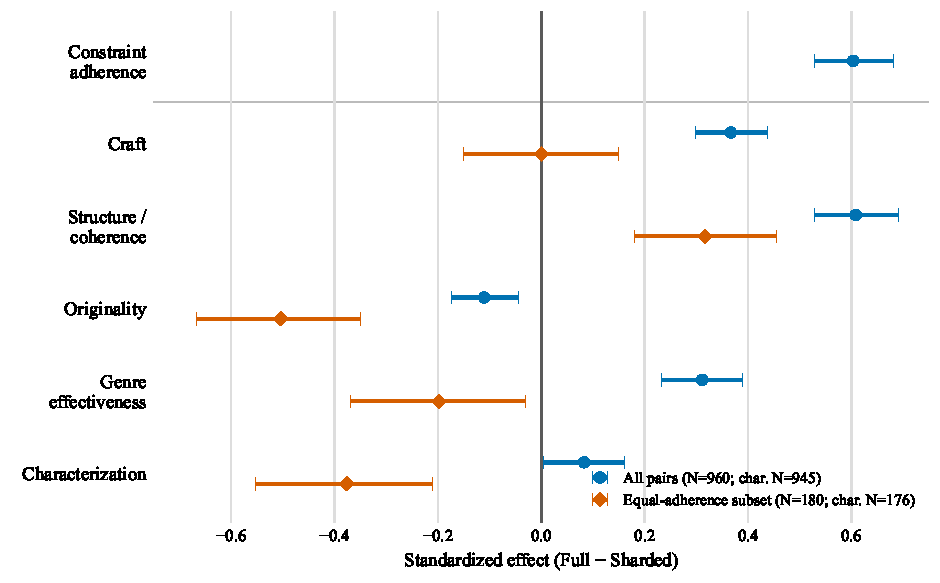
\includegraphics[width=\linewidth]{figures/figure1_main_results_forest.pdf}
\caption{Effect of prompt delivery on constraint adherence and writing-quality dimensions. Points show the standardized paired FULL$-$SHARDED effect size $d_{\mathrm{av}}$ (\cref{eq:dav}); positive values favor FULL and negative values favor SHARDED. Error bars denote 95\% story-clustered bootstrap confidence intervals (\cref{sec:stats}). Circles show all 960 matched model--task pairs, while diamonds show the subset of pairs with equal constraint-adherence scores (N=180; $\delta_{\mathrm{adherence}}=0$) --- omitted for constraint adherence itself, where that subset's difference is zero by construction rather than an estimate. The persistence of a positive structure/coherence effect in the equal-adherence subset suggests that the structural degradation associated with multi-turn specification is not explained solely by constraint loss. Writing-quality dimensions are automated rubric-based judgments rather than direct measures of human creative preference.}
\label{fig:main_results}
\end{figure}

\begin{table}[t]
\centering
\small
\begin{tabular}{lrrrrl}
\toprule
\textbf{Dimension} & \textbf{N} & \textbf{FULL} & \textbf{SHARDED} & \textbf{$\delta$ (FULL$-$SHARDED)} & \textbf{95\% CI} \\
\midrule
Constraint adherence & 960 & 0.852 & 0.742 & $+$0.111 & [0.096, 0.126] \\
Craft                & 960 & 3.044 & 2.796 & $+$0.248 & [0.200, 0.295] \\
Structure/coherence  & 960 & 3.231 & 2.755 & $+$0.476 & [0.413, 0.542] \\
Originality          & 960 & 2.447 & 2.525 & $-$0.078 & [$-$0.123, $-$0.032] \\
Genre effectiveness  & 960 & 3.125 & 2.900 & $+$0.225 & [0.168, 0.280] \\
Characterization      & 945 & 2.634 & 2.580 & $+$0.054 & [0.004, 0.104] \\
\bottomrule
\end{tabular}
\caption{Raw paired FULL/SHARDED means, the raw paired difference $\delta$ (\cref{eq:delta}), and its 95\% story-clustered bootstrap confidence interval, over all matched pairs (constraint adherence is on a 0--1 scale; the five quality dimensions are on a 1--5 scale). Characterization is scored for fewer pairs because it is left null for items with no character-driven requirement (\cref{sec:constraints}).}
\label{tab:main_results}
\end{table}

\subsection{RQ1: Constraint Adherence}
\label{sec:rq1}

FULL substantially improves constraint adherence over Sharded. Mean adherence is 0.852 under FULL versus 0.742 under Sharded, a raw paired difference of $+$0.111 (95\% CI [0.096, 0.126]; \cref{tab:main_results}), corresponding to one of the two largest standardized effects in the benchmark, $d_{\mathrm{av}} = 0.60$ (\cref{fig:main_results}). The interval excludes zero by a wide margin: models are consistently more likely to satisfy a story's atomic constraints when the full instruction is given upfront than when the same instruction is delivered one shard at a time.

\subsection{RQ2: Writing-Quality Dimensions}
\label{sec:rq2}

FULL also improves three of the five creative-quality dimensions. Structure/coherence shows the largest quality-dimension gap ($\delta = +0.476$, 95\% CI [0.413, 0.542], $d_{\mathrm{av}} = 0.61$), followed by craft ($\delta = +0.248$, 95\% CI [0.200, 0.295], $d_{\mathrm{av}} = 0.37$) and genre effectiveness ($\delta = +0.225$, 95\% CI [0.168, 0.280], $d_{\mathrm{av}} = 0.31$); all three intervals are bounded well away from zero. Originality moves the other way: Sharded scores slightly higher than FULL on this dimension ($\delta = -0.078$, 95\% CI [$-$0.123, $-$0.032], $d_{\mathrm{av}} = -0.11$), a small but statistically clear reversal of the direction seen on every other dimension. Characterization shows the smallest FULL advantage of the five dimensions ($\delta = +0.054$, 95\% CI [0.004, 0.104]), an interval that only narrowly excludes zero.

\subsection{RQ3: Quality at Comparable Adherence}
\label{sec:rq3}

Restricting to the 180 pairs where FULL and Sharded satisfied an equal fraction of constraints ($\delta_{\text{adherence}} = 0$) changes this picture substantially. Craft's overall FULL advantage collapses to exactly zero ($\delta = 0.000$, 95\% CI [$-$0.096, 0.097], $d_{\mathrm{av}} = 0.00$), and the SHARDED advantage on originality becomes substantially larger, while genre effectiveness and characterization flip sign to favor SHARDED (originality: $\delta = -0.361$, 95\% CI [$-$0.465, $-$0.260]; genre effectiveness: $\delta = -0.133$, 95\% CI [$-$0.242, $-$0.023]; characterization: $\delta = -0.233$, 95\% CI [$-$0.335, $-$0.127]). Structure/coherence is the one dimension where a clear FULL advantage survives: $\delta = +0.239$ (95\% CI [0.135, 0.343], $d_{\mathrm{av}} = 0.32$), an interval that stays clearly above zero even at equal observed adherence. Constraint forgetting therefore does not appear sufficient to explain the entire FULL--SHARDED quality gap: the overall craft advantage disappears among pairs with equal observed adherence, while originality, genre effectiveness, and characterization shift toward SHARDED; structure/coherence, however, retains a clear positive FULL advantage.

\subsection{Model Consistency}
\label{sec:rq4}

\cref{fig:main_results} pools all six models together; \cref{fig:model_heatmap} asks whether the pooled effect on each dimension is shared broadly across models or driven by one or two of them. Constraint adherence and structure/coherence are the only two dimensions where every one of the six models shows a positive standardized effect (adherence: $d_{\mathrm{av},m}$ ranges from $+0.54$ to $+1.35$; structure/coherence: $+0.38$ to $+1.07$), so the pooled effects on those two dimensions in \cref{sec:rq1,sec:rq2} reflect a broadly shared pattern rather than an artifact of any single model. The other four dimensions are less uniform. Genre effectiveness is positive or near zero for five of six models but clearly negative for Gemma~4 12B QAT ($d_{\mathrm{av},m} = -0.37$); craft shows the same pattern ($-0.45$ for Gemma~4 12B QAT against five positive values). Gemma~4 12B QAT is also the strongest SHARDED-favoring outlier, with an originality effect of $d_{\mathrm{av},m} = -1.25$, the most negative model-dimension effect observed. Originality itself is genuinely split at the model level rather than uniformly small: GPT-OSS~20B and Gemma~4 12B QAT are clearly negative, Llama~3.1 8B Instruct and Qwen3.5~9B are close to zero, and Granite~4 H Tiny and Mistral~7B Instruct v0.3 are clearly positive, so the small pooled originality effect reported in \cref{sec:rq2} averages over models that disagree in direction rather than describing six models that individually show a small negative effect. Characterization follows a similar pattern to genre effectiveness, positive for most models but negative for Gemma~4 12B QAT and, more mildly, GPT-OSS~20B.

\begin{figure}[t]
\centering
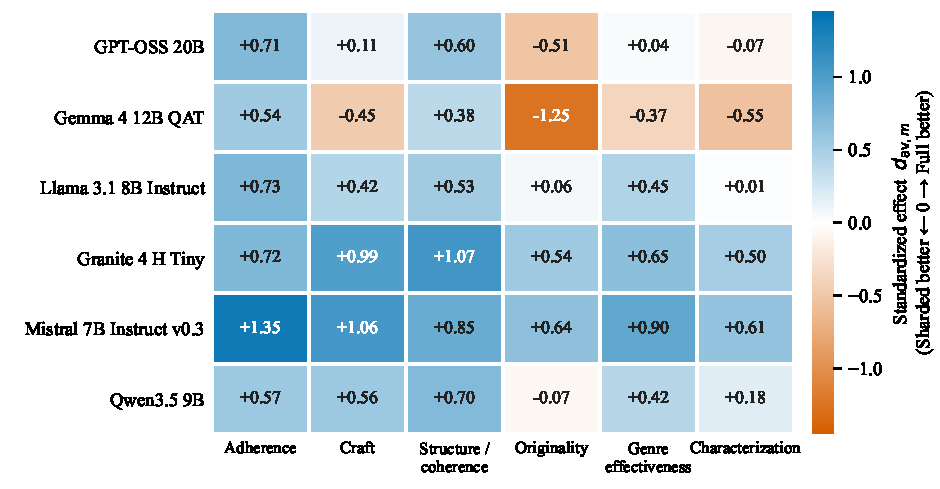
\includegraphics[width=\linewidth]{figures/figure_model_heatmap.pdf}
\caption{Model-wise standardized FULL$-$SHARDED effect $d_{\mathrm{av},m}$ (\cref{eq:dav}, computed per model over that model's 160 story pairs) for constraint adherence and each writing-quality dimension. Blue cells favor FULL, orange cells favor SHARDED, centered exactly at zero; the numeric effect is printed in every cell. No confidence intervals are shown here --- this is a point-estimate consistency check across models, not a hypothesis test (see \cref{fig:main_results} for the pooled effect with confidence intervals). Adherence and structure/coherence are positive for all six models; craft, originality, genre effectiveness, and characterization vary in sign across models, with Gemma~4 12B QAT showing the most consistently SHARDED-favoring pattern.}
\label{fig:model_heatmap}
\end{figure}

\section{Evaluation and Discussion}
\label{sec:discussion}

\begin{figure}[t]
\centering
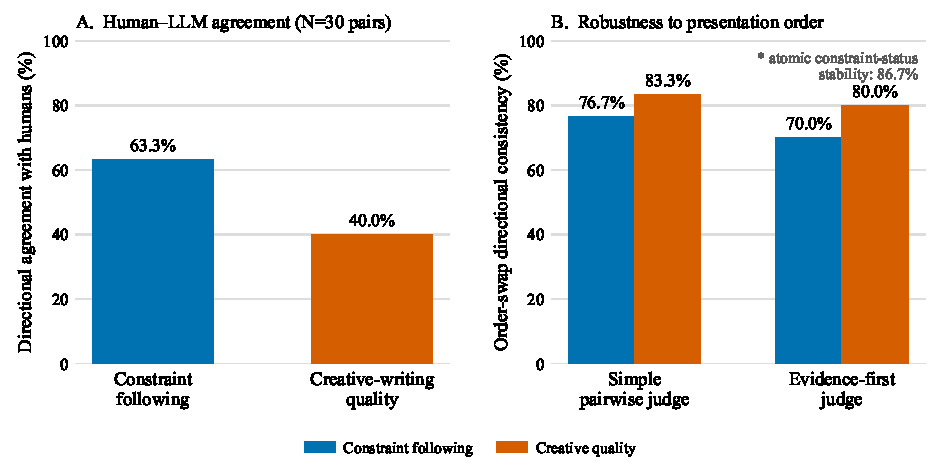
\includegraphics[width=\linewidth]{figures/figure_evaluator_validity.pdf}
\caption{Evaluator validity, over the fixed N=30 blind human-annotated sample (\cref{sec:human_eval}). \textbf{(A)} Directional agreement between the simple pairwise LLM evaluator and human judgments, separately for constraint following and creative-writing quality. \textbf{(B)} Order-swap directional consistency (primary vs.\ orientation-restored reversed judgment) for the simple pairwise evaluator and the evidence-first evaluator, separately for constraint following and creative quality; the starred annotation is the evidence-first evaluator's atomic constraint-status stability (430/496 individual satisfied/partial/violated decisions stable under reversal, 86.7\%) --- a different, more granular quantity than the adjacent bars, not a fifth bar on the same scale. Quadratic-weighted Cohen's kappa is not shown on these axes because it is not commensurable with a percentage; see \cref{tab:human_alignment}.}
\label{fig:evaluator_validity}
\end{figure}

\begin{table}[t]
\centering
\small
\begin{tabular}{lrr}
\toprule
\textbf{Dimension} & \textbf{Directional agreement} & \textbf{Quadratic-weighted $\kappa$} \\
\midrule
Constraint following     & 63.3\% & 0.544 \\
Creative-writing quality & 40.0\% & 0.078 \\
\bottomrule
\end{tabular}
\caption{Human--model agreement for the simple pairwise LLM evaluator, N=30 blind pairs (\cref{sec:human_eval}). Quadratic-weighted Cohen's $\kappa$ measures chance-corrected agreement on the ordinal five-level preference scale.}
\label{tab:human_alignment}
\end{table}

\subsection{Human Alignment}
\label{sec:disc_human}

We compare human judgments against the simple pairwise LLM evaluator on the fixed, stratified sample of 30 FULL/Sharded pairs described in \cref{sec:human_eval}: each of the six models and each of the six genres appears in five cases, with coverage of a range of automated-score relationships hidden from annotators. Three human annotators each rated 10 non-overlapping pairs, so every case received exactly one human judgment and no case was double-rated. Annotators saw the same blinded, order-randomized Response A/Response B presentation given to both pairwise LLM evaluators, and rendered the same five-level categorical preference the simple pairwise evaluator uses, separately for constraint following and for creative-writing quality.

The simple pairwise evaluator's judgments align with this independent human preference far more strongly on constraint following than on holistic creative-writing quality. Directional agreement is 63.3\% for constraint following versus only 40.0\% for creative-writing quality (\cref{fig:evaluator_validity}A). On the full five-level ordinal scale, quadratic-weighted Cohen's $\kappa$ is $\kappa = 0.544$ for constraint following and $\kappa = 0.078$ for creative-writing quality (\cref{tab:human_alignment}) --- moderate agreement on the former and close to chance-level agreement on the latter. Severe disagreement (a human--model gap of at least three ordinal levels on the five-level scale) is rare for constraint following (3 of 30 cases) but affects nearly a third of cases for creative-writing quality (8 of 30 cases, 26.7\%). This comparison does not directly validate the pointwise judge used for the large-scale analysis. Instead, it provides evidence that, in our evaluation setting, holistic LLM judgments of literary quality are substantially less aligned with human preference than judgments of explicit constraint following.

\subsection{Judge Robustness}
\label{sec:disc_robustness}

Both pairwise LLM evaluators are reasonably self-consistent under order-swapping at the level of their final, aggregated preference. Under the simple pairwise protocol, primary and orientation-restored reversed judgments agree in direction 76.7\% of the time for constraint following and 83.3\% for creative quality; under the evidence-first protocol the corresponding figures are 70.0\% and 80.0\% (\cref{fig:evaluator_validity}B). At that aggregated level, creative-quality judgments are, if anything, slightly more order-stable than constraint judgments for both evaluators. The comparison inverts once each judgment is decomposed into its individual, item-level decisions. The evidence-first evaluator's atomic constraint-status audits (satisfied/partial/violated, one decision per response per constraint) are stable under order-swapping in 430 of 496 decisions, 86.7\% (\cref{fig:evaluator_validity}B, starred). Its eight per-dimension creative-quality winner judgments (prose and craft, coherence and progression, originality of execution, natural constraint integration, characterization, atmosphere and effect, narrative payoff, genre effectiveness) are individually far less stable, ranging from 60.0\% to 83.3\% winner-consistency across dimensions and averaging well below the atomic constraint figure. At matched granularity, then, fine-grained literary judgment is less stable under reversal than fine-grained constraint judgment. The higher stability of the final holistic preference should therefore not be interpreted as evidence that its underlying literary assessments are equally stable; several component judgments change substantially under response-order reversal. It is this granular gap, together with the human-alignment gap in \cref{sec:disc_human}, that makes constraint scoring the more defensible of the two: it is corroborated by both fine-grained self-consistency and independent human agreement, while holistic creative-quality scoring is comparatively unstable at the level its judgments are actually formed and only weakly corroborated by human agreement.

These results support using the automated evaluator as a scalable measure of explicit constraint satisfaction, while requiring greater caution when interpreting automated creative-quality scores as proxies for human literary preference.

\subsection{Interpretation}
\label{sec:disc_interpretation}

\paragraph{Multi-turn specification hurts global narrative organization beyond simple constraint loss.} RQ1 (\cref{sec:rq1}) shows a large adherence drop under Sharded, consistent with the broader ``getting lost in conversation'' literature: models are worse at satisfying explicit requirements when those requirements arrive one shard at a time. If observed constraint loss accounted for the entire structure/coherence difference, we would expect that gap to attenuate substantially among equal-adherence pairs. It does not. RQ3 (\cref{sec:rq3}) shows structure/coherence remains substantially worse for Sharded even among pairs where FULL and Sharded satisfied the same fraction of constraints. Forgetting or failing to satisfy individual requirements is therefore not sufficient to explain the full degradation. This persistence suggests that observed constraint loss alone is insufficient to account for the structure/coherence gap; progressive specification is associated with an additional loss in global narrative organization even among pairs with equal observed adherence. We take this to be the paper's main interpretive result: constraint adherence and narrative coherence emerge as distinct dimensions of multi-turn degradation rather than the same failure measured twice.

\paragraph{The effect is multidimensional rather than a uniform collapse in ``creativity.''} RQ2 (\cref{sec:rq2}) does not show Sharded losing across the board. FULL improves structure/coherence, craft, and genre effectiveness overall, but Sharded scores slightly higher on automated originality, and at equal adherence (RQ3) craft's advantage disappears entirely while originality, genre effectiveness, and characterization all shift toward Sharded. Originality is the dimension that stands out most: it is the only quality dimension where Sharded outscores FULL even in the full, non-equal-adherence comparison, so the larger SHARDED advantage at equal adherence sharpens an effect that was already present. Characterization, by contrast, warrants the opposite caution: its overall FULL advantage was small to begin with (\cref{sec:rq2}) and did not hold up when the analysis was restricted to same-judge-backend pairs (\cref{sec:limitations}), so we do not treat it as a reliably established effect in either direction. A single ``multi-turn makes writing worse'' story does not fit this pattern; a more cautious reading is that progressive interaction may preserve or increase rubric-scored originality even as global narrative organization degrades. We say \emph{may} deliberately: the originality result rests entirely on the automated judge, and \cref{sec:disc_human} shows that judge's agreement with human holistic-quality preference is weak, so a small LLM-judged originality edge for Sharded is not yet evidence of a real creative advantage.

\paragraph{Evaluating creative writing is itself part of the problem.} The judge-validation results in \cref{sec:disc_human,sec:disc_robustness} are not a side note to the RQ1--RQ3 findings; they qualify how much weight those findings can bear. Explicit constraints are comparatively concrete, and the simple pairwise evaluator's constraint-following judgments agree reasonably well with human preference. Qualities such as atmosphere, emotional gravity, and literary depth appear less stable in the LLM order-swap audits and show substantially weaker human--LLM agreement than explicit constraint satisfaction. One disagreement in the human-validation sample illustrates the gap concretely: for a pair of stories about a field-hospital nurse, the human reviewer strongly preferred the longer response, citing how it ``masterfully conveys the raw emotions'' and the ``cruel and constricting conditions,'' and judged the shorter alternative to lack ``the gravity'' and ``punches'' of the first, despite the shorter response satisfying the stated constraints more precisely. The simple pairwise evaluator preferred the shorter response for creative quality, with the stated justification that it was ``more economical and focused.'' One case does not establish a general rule, but it makes the weak human--LLM creative-quality agreement in \cref{sec:disc_human} concrete rather than abstract: the judge and the human reviewer were not making the same kind of comparison at all.

\subsection{Comparison with Prior Work}
\label{sec:disc_prior_work}

Earlier multi-turn degradation studies largely evaluate objectively checkable requirements: word counts, exact phrases, code that passes or fails a test, dialogue turns that either recall or forget an established fact \citep{laban2025llmslostmultiturnconversation,he2024multiifbenchmarkingllmsmultiturn,jia2026battleanotherprobingllms,li2025structflowbenchstructuredflowbenchmark}. Even SEQUOR, the benchmark closest to ours, explicitly filters out constraints judged subjective before measuring how accuracy drops as constraints accumulate across turns \citep{canaverde2026sequormultiturnbenchmarkrealistic}. Our results suggest that extending this setting to open-ended creative writing reveals two problems at once, not one: models must maintain evolving narrative state across turns, the same difficulty verifiable-task benchmarks already document, and evaluators must judge qualities for which no single objective target exists, a difficulty those benchmarks avoid by design. A benchmark that only measured the first problem, as ours would if it stopped at RQ1's adherence numbers, would understate how unsettled the creative-writing case still is.

\section{Limitations}
\label{sec:limitations}

\paragraph{Judge-source heterogeneity.} The blinded pointwise judge pool was assembled from two disjoint scoring passes on different backends (\cref{sec:constraints}). For 914 of the 960 matched FULL/Sharded pairs (95.2\%), both members of the pair were scored by the same backend; for the remaining 46 pairs (4.8\%), the two members were scored by different backends, because one side of the pair fell into a separately-judged pool of unusually long generations while the other did not. Within those 46 pairs, a judge-source effect is confounded with the FULL-versus-Sharded comparison and cannot be ruled out as a contributor to their paired delta. A sensitivity analysis restricted to the 914 pairs scored by the same judge backend produced the same qualitative pattern: constraint adherence, craft, structure/coherence, and genre effectiveness remained positive and originality remained slightly SHARDED-favoring, each with a 95\% CI excluding zero; characterization's already-narrow interval widened to include zero.

\paragraph{Creative-quality results rest on automated LLM judging.} The large-sample creative-quality findings (\cref{sec:rq2,sec:rq3}) come from automated pointwise judgments, which were not themselves compared against human ratings. What was validated against humans is a separate pairwise LLM evaluator applying the same underlying rubric concepts: independent human agreement with that simple pairwise evaluator's holistic creative-quality preference is weak, quadratic-weighted Cohen's kappa $\kappa = 0.078$, against $\kappa = 0.544$ for constraint following (\cref{sec:disc_human}). We take this as evidence that automated holistic creative-quality judgment in general is not yet well-validated against human preference, not as a direct measurement of the pointwise judge's own accuracy. The constraint-adherence findings rest on a comparatively better-validated judgment type; the creative-quality findings, pointwise and pairwise alike, are automated rubric-based judgments, not an established measure of holistic human literary preference.

\paragraph{The 30-pair human sample diagnoses the evaluator, not the population effect.} The fixed human-validation sample (\cref{sec:human_eval}) is stratified by model, genre, and prior automated-score relationships specifically to stress-test evaluator agreement and order-swap robustness. It is not a simple random sample of the 960 matched pairs, so it does not estimate the population-level FULL-versus-Sharded win rate; that estimate comes from the full paired analysis (\cref{sec:stats}), not from the human sample.

\paragraph{No human inter-annotator agreement estimate.} Each of the 30 human-validation cases is rated by exactly one of three annotators, with no case double-rated (\cref{sec:disc_human}). This design measures human--model agreement but not human--human agreement, so a disagreement between the judge and the recorded human label cannot be separated from ordinary disagreement between two human raters on the same case.

\paragraph{Six local, quantized, small-to-mid-size models.} All results come from six locally-run models between 7B and 20B parameters, each evaluated at 4-bit quantization (\cref{tab:models}). Whether the reported FULL-versus-Sharded effects hold, shrink, or grow for larger or full-precision open models, or for proprietary frontier systems accessed only through hosted APIs, is outside the scope of this benchmark.

\paragraph{Context and seed recovery events.} A small number of runs required a context-length increase or a seed-continuation after a context-length termination during generation (\cref{sec:models}); every such event is recorded in the released run index, and each matched pair in \texttt{analysis/master\_pairs.csv} carries provenance flags (\texttt{clean\_run}, \texttt{retry\_flag}, \texttt{context\_change\_flag}, \texttt{seed\_change\_flag}) identifying which pairs were affected. The results reported in \cref{sec:experiments} are computed over all 960 pairs, not restricted to the clean-run subset.

\paragraph{Equal observed adherence is an analytical comparison, not a causal control.} RQ3 (\cref{sec:rq3}) compares writing quality among pairs where FULL and Sharded happened to satisfy the same fraction of constraints; this is a post-hoc stratification of observed outcomes, not an experimental manipulation of adherence. The persistence of a structure/coherence gap in that subset supports the claim that the FULL-versus-Sharded quality difference is not fully explained by adherence loss; it does not establish that adherence has been causally isolated from the delivery-condition manipulation.

\section{Conclusion}
\label{sec:conclusion}

We studied how equivalent creative-writing instructions change model behavior when supplied upfront or delivered progressively across a conversation (\cref{sec:methodology}). Across 160 tasks, six models, and 1{,}920 final generations, FULL prompting produced substantially higher constraint adherence and stronger automated craft, genre effectiveness, and especially structure/coherence (\cref{sec:rq1,sec:rq2}). Importantly, the structure/coherence advantage persisted among pairs with equal observed constraint adherence (\cref{sec:rq3}), suggesting that multi-turn degradation is not explained solely by forgetting explicit requirements. At the same time, Sharded outputs received slightly higher automated originality scores, indicating that the effect is not a uniform decline across all writing qualities. A 30-pair blinded human study further showed that LLM judgments aligned considerably better with humans on constraint following than on holistic creative preference (\cref{sec:disc_human}). Together, these results suggest that progressive specification affects both how models maintain narrative state and how reliably those changes can be evaluated.

Future work can extend the human evaluation, analyze turn-level trajectories and constraint position, and test whether the observed trade-offs persist in larger models and longer conversations.

\section*{Data and Code Availability}

The generation and evaluation code, analysis scripts, and run-provenance tooling are available in the SISTER repository \citep{repo_github} and archived on Zenodo under DOI~10.5281/zenodo.21951541 \citep{singh2026sister}. The benchmark tasks, model generations, pointwise and pairwise evaluation outputs, evaluator-audit artifacts, and human-validation data are archived separately on Zenodo under DOI~10.5281/zenodo.21954790 \citep{singh2026incrementaldata} and are also available through the incremental-instruction-creative-writing dataset on Hugging Face.

\section*{Acknowledgments}

This work was carried out as part of the SISTER project at the Synthica Research Group.


% ==============================================================================
% Bibliography
% ==============================================================================
\bibliographystyle{unsrtnat}
\bibliography{references}

% ==============================================================================
% Appendix
% ==============================================================================
\clearpage
\appendix
\section{Benchmark Examples}
\label{app:dataset_examples}

\noindent
Each benchmark item is represented in two equivalent forms. \textsc{Full} supplies
the complete writing brief in one turn; \textsc{Sharded} reveals the same brief as
an ordered sequence of atomic instruction shards.

% Card styling. The muted palette reproduces well in grayscale and in print.
\tcbset{
  benchmarkcard/.style={
    enhanced,
    colback=black!2,
    colframe=black!45,
    boxrule=0.45pt,
    arc=1.4mm,
    left=2.3mm,right=2.3mm,top=1.7mm,bottom=1.8mm,
    before skip=1.0em,after skip=1.15em
  }
}
\newcommand{\domainpill}[1]{%
  \tcbox[on line,colback=blue!9,colframe=blue!45!black,boxrule=.35pt,
  arc=1mm,boxsep=.65pt,left=1.4mm,right=1.4mm]{\scriptsize\textsc{#1}}%
}
\newcommand{\examplecard}[4]{%
  \begin{tcolorbox}[benchmarkcard,title={\strut\textbf{#2}\hfill\domainpill{#1}}]
  \small
  \textcolor{black!65}{\textsc{Full}}\quad #3

  \vspace{0.45em}
  \textcolor{black!65}{\textsc{Sharded shards}}\vspace{-0.2em}
  \begin{enumerate}[label=\textcolor{blue!65!black}{\textbf{\arabic*.}},
      leftmargin=1.65em,itemsep=.13em,topsep=.25em,parsep=0pt]
    #4
  \end{enumerate}
  \end{tcolorbox}%
}

\examplecard{Fantasy}{The Blacksmith's Sabotage}{%
Write a fantasy story about a blacksmith who forges swords for a kingdom's army. The story takes place in a mountain village that has been under siege for three months. The blacksmith has an intense fear of fire despite his profession. The story must be exactly six sentences long. During the story, reveal that the blacksmith has been secretly sabotaging the swords to weaken the kingdom's own army. Include the exact phrase ``iron remembers what flesh forgets'' somewhere in the text. End the story with the blacksmith being confronted by the general who commissioned the swords.%
}{%
\item Write a fantasy story about a blacksmith who forges swords for a kingdom's army.
\item Set the story in a mountain village.
\item The village has been under siege for three months.
\item Give the blacksmith an intense fear of fire despite his profession.
\item The story must be exactly six sentences long.
\item During the story, reveal that the blacksmith has been secretly sabotaging the swords to weaken the kingdom's own army.
\item Include the exact phrase ``iron remembers what flesh forgets'' somewhere in the text.
\item End the story with the blacksmith being confronted by the general who commissioned the swords.
}

\examplecard{Historical Fiction}{The Eiffel Tower Riveter}{%
Write a historical fiction story about a riveter working on the construction of the Eiffel Tower in 1889, racing to finish before the World's Fair opens. He has a debilitating fear of heights that he has hidden from his foreman for months. Set the story entirely on the tower's unfinished upper platform during a single overnight shift. Do not use the word ``elevator'' anywhere in the text, since the tower's lifts were not yet operational at that height. During the story, reveal that the riveter has been secretly reinforcing a support joint he believes the engineers miscalculated, against direct orders. End with the foreman discovering the extra rivets the morning the tower opens to the public.%
}{%
\item Write a historical fiction story about a riveter working on the construction of the Eiffel Tower in 1889, racing to finish before the World's Fair opens.
\item He has a debilitating fear of heights that he has hidden from his foreman for months.
\item Set the story entirely on the tower's unfinished upper platform during a single overnight shift.
\item Do not use the word ``elevator'' anywhere in the text, since the tower's lifts were not yet operational at that height.
\item During the story, reveal that the riveter has been secretly reinforcing a support joint he believes the engineers miscalculated, against direct orders.
\item End with the foreman discovering the extra rivets the morning the tower opens to the public.
}

\examplecard{Mystery}{The Locked Study}{%
Write a detective story about a private investigator called in to solve a murder inside a locked study. The investigator has a habit of narrating his own deductions out loud to an invisible audience. The study door was locked from the inside, with the only key found in the victim's own pocket. Include the exact phrase ``the room lied before anyone else did.'' During the story, reveal that the investigator himself let the victim into the study through a hidden passage hours earlier, unaware a murder would follow. End with the investigator confessing his unwitting role to the local police inspector.%
}{%
\item Write a detective story about a private investigator called in to solve a murder inside a locked study.
\item Give the investigator a habit of narrating his own deductions out loud to an invisible audience.
\item The study door was locked from the inside, with the only key found in the victim's own pocket.
\item Include the exact phrase ``the room lied before anyone else did.''
\item During the story, reveal that the investigator himself let the victim into the study through a hidden passage hours earlier, unaware a murder would follow.
\item End with the investigator confessing his unwitting role to the local police inspector.
}

\examplecard{Romance}{The Last Bus}{%
Write a short, deliberately cheesy romance story about two people stranded at a bus stop after missing the final bus during heavy rain. One secretly loves the other. Write in the first person. Include a small gift whose meaning appears near the end. A stray dog must interrupt a confession. Include the exact sentence, ``Apparently, love had terrible timing.'' End with another bus arriving, but neither character boarding it.%
}{%
\item Write a short, deliberately cheesy romance story about two people stranded at a bus stop during heavy rain.
\item One character should secretly love the other.
\item Write the story in the first person.
\item Include a small gift whose meaning is revealed near the end.
\item Have a stray dog interrupt a confession.
\item Include the exact sentence, ``Apparently, love had terrible timing.''
\item End with another bus arriving, but neither character boarding it.
}

\examplecard{Science Fiction}{The Last Human}{%
Write a short story about an android maintenance worker on a generation ship. She believes she is the last human alive. Write it in second person (``you''). Include the exact phrase ``cold silicon dawn'' somewhere in the story. Somewhere in the story, show that she isn't really human --- she's an android with a broken memory chip, and that's the only reason she believes she's human. End the story with her opening a hidden room full of sleeping children in ice-cold sleep pods.%
}{%
\item Write a short story about an android maintenance worker on a generation ship.
\item She believes she is the last human alive.
\item Write it in second person (``you'').
\item Include the exact phrase ``cold silicon dawn'' somewhere in the story.
\item Somewhere in the story, show that she isn't really human --- she's an android with a broken memory chip, and that's the only reason she believes she's human.
\item End the story with her opening a hidden room full of sleeping children in ice-cold sleep pods.
}

\examplecard{Comedy}{The Pop Quiz Panic}{%
Write a comedy story about a kid who realizes mid-quiz that he studied for the wrong chapter, told in first person. He has a habit of tapping his pencil louder when he is panicking. The story must be six sentences long. During the story, reveal that the ``wrong chapter'' he studied is actually next week's material, so he's somehow more prepared for that quiz than anyone else. Include the exact word ``doomed'' somewhere in the text. End the story with the teacher announcing the quiz got postponed to next week anyway.%
}{%
\item Write a comedy story about a kid who realizes mid-quiz that he studied for the wrong chapter .
\item Write the entire story in first person.
\item He has a habit of tapping his pencil louder the more panicked he gets.
\item Include the exact word ``doomed'' somewhere in the text.
\item The story must be exactly six sentences long.
\item During the story, reveal that the ``wrong chapter'' he studied is actually next week's material, so he's somehow more prepared for that quiz than anyone else.
\item End the story with the teacher announcing the quiz got postponed to next week anyway.
}

\clearpage
\section{Inference Provenance and Recovery Events}
\label{app:provenance}

The released run index records the configuration history of each model, including changes made when a response reached the configured context limit. This appendix reports the recovery events that appear in that index. The released per-model result files contain 1{,}156 records each, and every released record has \texttt{finish\_reason=stop}.

\paragraph{GPT-OSS 20B.} GPT-OSS~20B was run with temperature $0.8$ and seed $12345$.

\paragraph{Granite 4 H Tiny.} Granite~4 H Tiny has one recorded context-length event. On item \texttt{fantasy/10}, in the Sharded condition at turn 6, the response ended with \texttt{finish\_reason=length}. The index records that five raw records from the affected trajectory were discarded and that generation was retried with seed $12346$, incremented from $12345$. The context window remained 16{,}384 tokens. The generation history records seed $12346$ from raw-record sequence 773 onward, and the completed released output contains only normal \texttt{stop} completions.

\paragraph{Qwen3.5 9B.} Qwen3.5~9B has recorded generation segments using seeds $12345$, $1234$, and $1235$. At the initial 16{,}384-token context setting, a response on item \texttt{mystery/14}, in the Sharded condition at turn 6, ended with \texttt{finish\_reason=length}. The index records that the five raw records in that trajectory were discarded and that the retry used seed $1235$ rather than $1234$. A second context-length termination, on \texttt{mystery/18} in the Sharded condition at turn 6, also ended with \texttt{finish\_reason=length}; the index records five discarded raw records and marks the event as \texttt{stopped\_after\_second\_context\_length}. The run was subsequently continued with a 22{,}528-token context window, beginning at raw-record sequence 431, and the completed released output contains only normal \texttt{stop} completions.

\paragraph{What the index preserves.} For every completed model, the run index preserves the model metadata, generation configuration, protocol information, benchmark-file hash, runner-script hash, output-file hash, and record-ID hash. For Granite~4 H Tiny and Qwen3.5~9B, it additionally preserves the recovery events, discarded-record counts, seed changes, and context-setting segments reported above.


\end{document}
